
\section{XZ Utils backdoor} % Sections are added in order to organize your presentation into discrete blocks, all sections and subsections are automatically output to the table of contents as an overview of the talk but NOT output in the presentation as separate slides

%------------------------------------------------

\begin{frame}
\frametitle{Cosa è successo?}

\begin{columns}
        \begin{column}{0.5\textwidth}
            \begin{itemize}
                \item Andres Freund, Microsoft software engineer, scopre un problema di sicurezza nella versione 5.6.[0-1] di XZ.
                \item La falla si dimostra essere una backdoor per eseguire codice arbitrario tramite una connessione SSH in corrispondenza di una chiave privata.
            \end{itemize}
        \end{column}
        \begin{column}{0.5\textwidth}
            \centering
            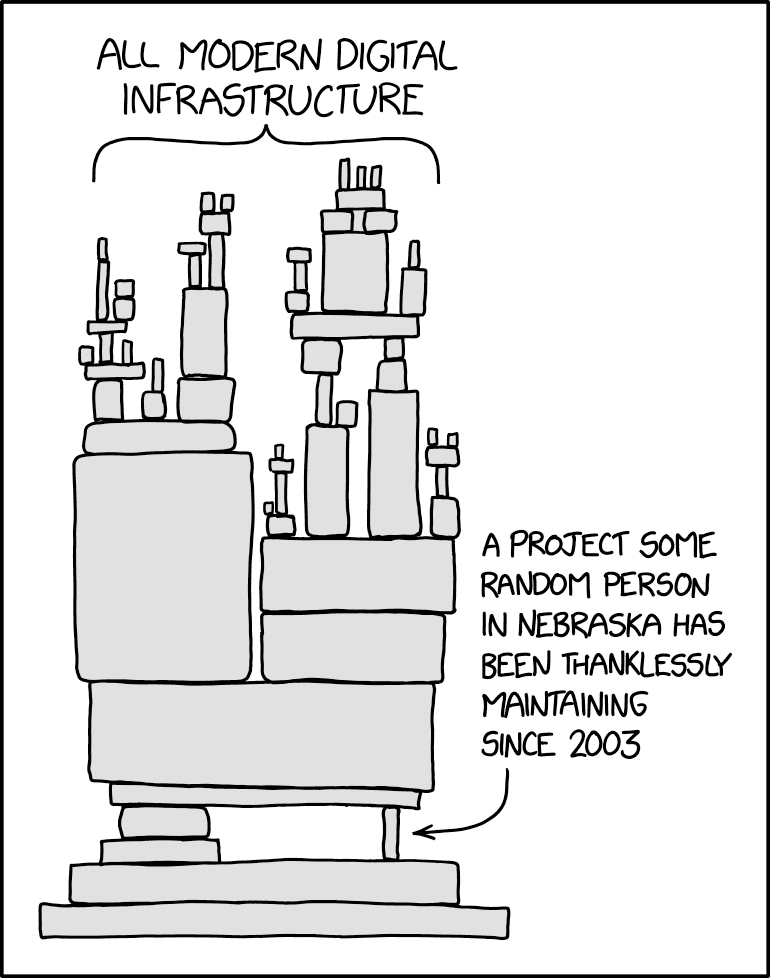
\includegraphics[width=\textwidth]{img/2-Introduction/dependency_2x.png}
        \end{column}
\end{columns}

\end{frame}


\begin{frame}
\frametitle{Supply-chain attacks}
Invece che attaccare direttamente l'agente SSH si è passato per una libreria utilizzata dalle sue dipendenze.

\vspace{1 cm}
\centering
    libzma e XZ $\rightarrow$ libsystemd $\rightarrow$ Systemd $\rightarrow$ SSH Agent

\end{frame}

\begin{frame}
\frametitle{Supply-chain attacks}

Un attacco alla supply chain è una strategia di attacco informatico che sfrutta strumenti o servizi di terze parti — collettivamente noti come "supply chain" — per infiltrarsi nel sistema o nella rete di un obiettivo.

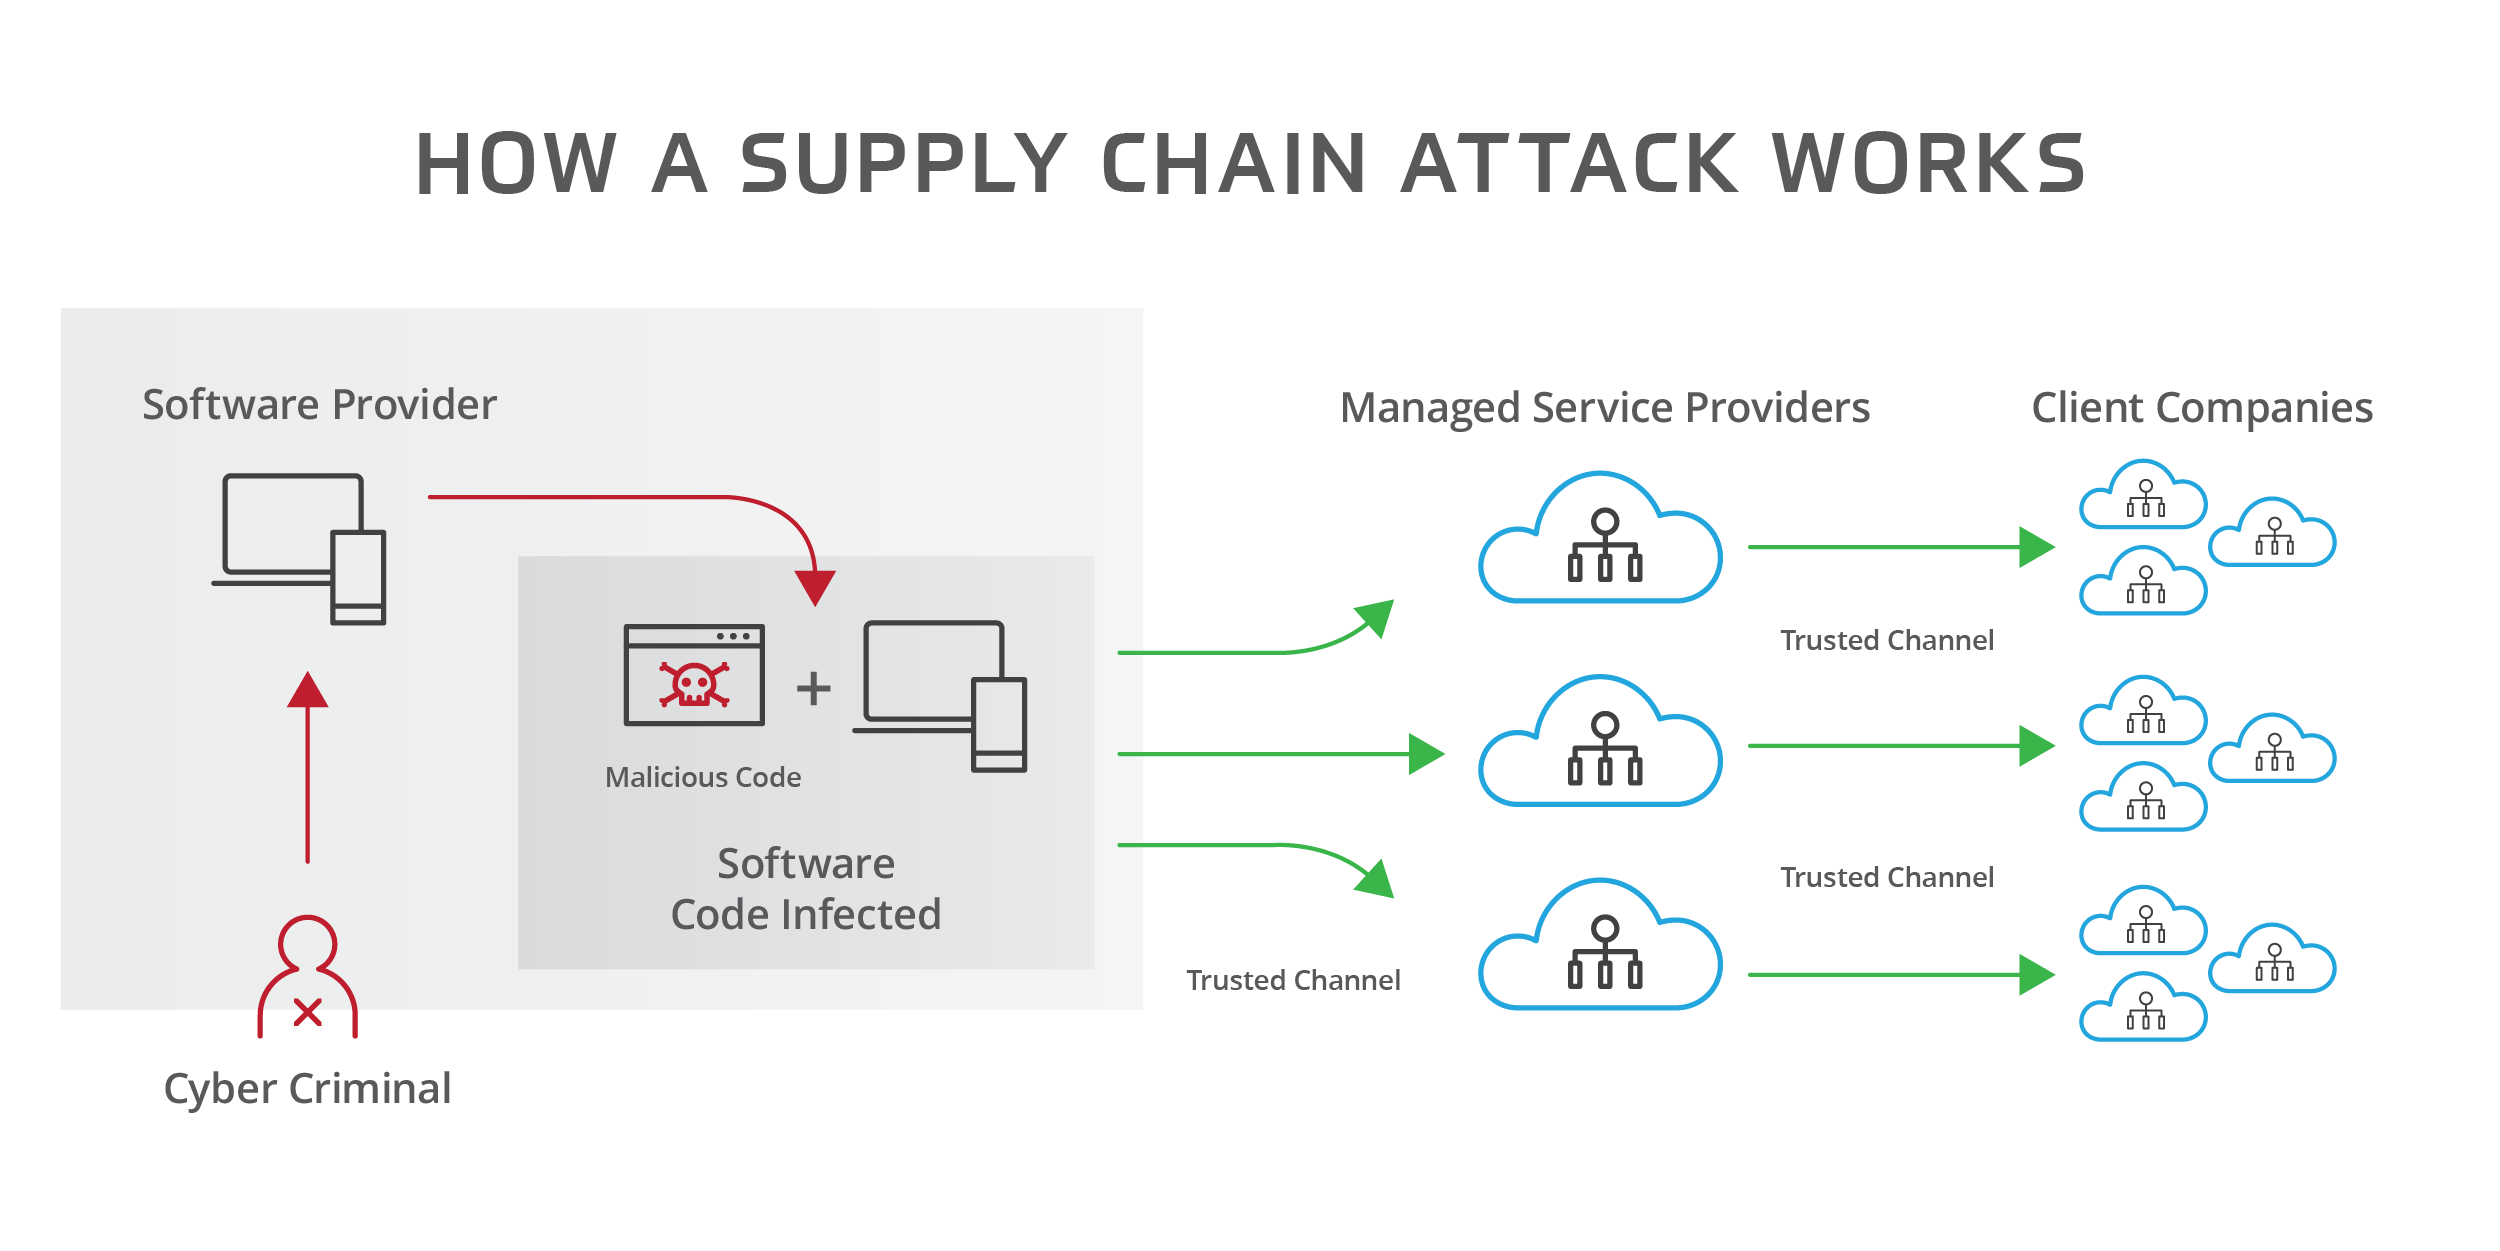
\includegraphics[width=0.8\textwidth]{img/2-Introduction/supplychain.png}
\end{frame}


\begin{frame}
\frametitle{Supply-chain attacks!}

Gli attacchi alla supply chain rappresentano una minaccia significativa poiché sfruttano la fiducia che le organizzazioni ripongono nei loro fornitori.
\begin{center}
  
\includegraphics[width=0.4\textwidth]{img/2-Introduction/Warning.jpg}  
\end{center}
    
\end{frame}

\begin{frame}
\frametitle{Ingegneria sociale e meltdown}
La backdoor XZ Utils è stata il culmine di circa \textbf{tre anni di sforzi} da parte dell'utente "Jia Tan" che ha tentato di \textbf{ottenere la fiducia del mantenitore} del progetto.

\vspace{0.5 cm}

Dopo un periodo di pressione, tramite l'utilizzo di \textbf{numerevoli account fantocci}, sul fondatore e manutentore del progetto, Jia Tan ha ottenuto la posizione di co-manutentore degli XZ Utils ed è stato in grado di approvare la versione 5.6.X della libreria contenente il malware.

\end{frame}

\begin{frame}
    \frametitle{Come Funziona la Vulnerabilità P2}
    \begin{itemize}
        \item La patch dormiente ha il compito di sostituire la funzione RSA\_public\_decrypt di OpenSSH con una versione malevola.
        \item OpenSSH normalmente non carica liblzma, ma una patch comune delle distribuzioni linux fa sì che venga caricata libsystemd, che a sua volta carica lzma.
        \item Una versione modificata di build-to-host.m4 nel tar file di rilascio estrae uno script che esegue l'iniezione nel liblzma.
    \end{itemize}
\end{frame}

\begin{frame}
    \frametitle{Peggore backdor della storia}
    \textbf{\textcolor{red}{Alex Stamos: "this could have been the most widespread and effective backdoor ever planted in any software product"}}.

    \begin{center}
        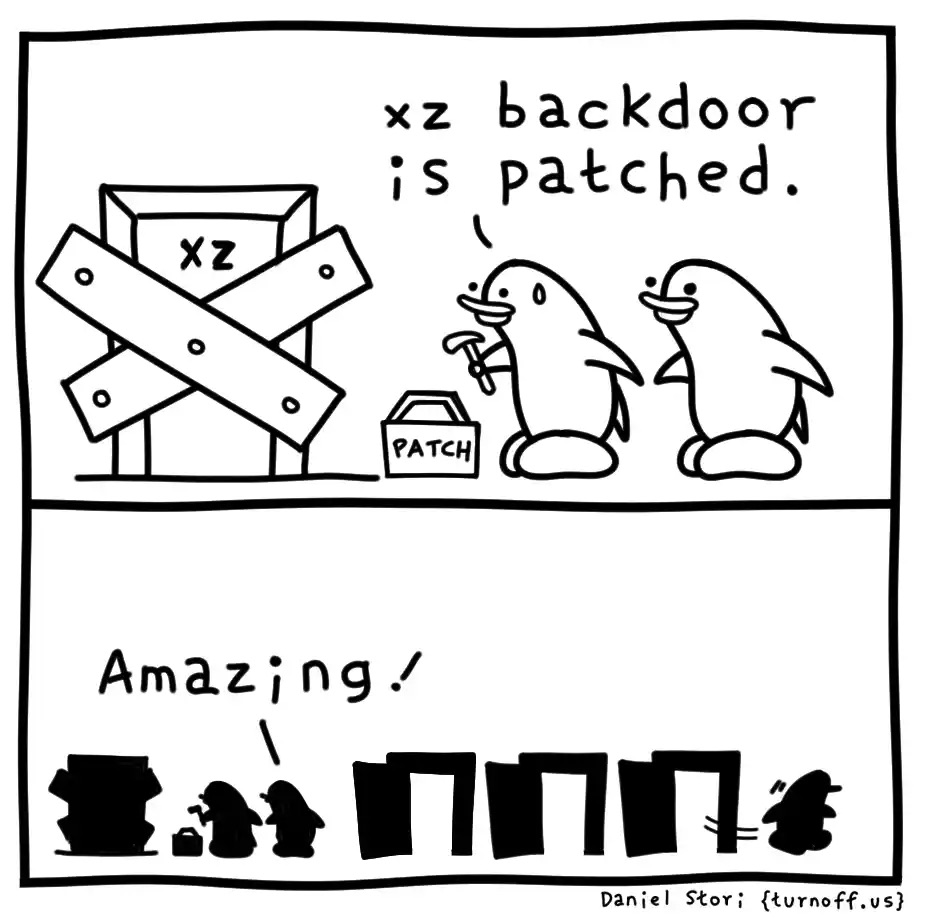
\includegraphics[width=0.4\linewidth]{img/2-Introduction/xz-backdoor-patched.jpeg}
    \end{center}
\vspace{0.5 cm}

\end{frame}